\section{留数定理应用}
\subsection{三角函数的积分}
考虑积分区间为$\left[ 0, 2\pi \right]$,被积函数为三角函数有理式的积分
\begin{equation}
    \int_{0}^{2\pi} R(\cos{x}, \sin{x}) dx,
\end{equation}
当实变数 $x$ 从 0 变到 $2 \pi$ 时, 复变数 $z=e^{\imath x}$ 从 $z=1$ 出发沿单位圆 $|z|=1$ 逆时针 走一圈又回到 $z=1$,
实变定积分化为复变回路积分, 就可以应用留数定理了. 至于实变定积分里的 $\cos x, \sin x$ 和 $d x$, 作如下变换:
$$
\cos x=\frac{1}{2}\left(z+z^{-1}\right), \quad \sin x=\frac{1}{2 \imath}\left(z-z^{-1}\right), \quad d x=\frac{1}{\imath z} d z .
$$
于是, 原积分化为
$$
I=\oint_{|z|=1} R\left(\frac{z+z^{-1}}{2}, \frac{z-z^{-1}}{2 \imath}\right) \frac{d z}{\imath z}
$$
利用留数定理即可求得.

\begin{examplebox}{求定积分\[I=\int_0^{2 \pi} \frac{d \theta}{1+a \cos \theta}, \quad|a|<1 \]}
    根据上面的方法,可得
    \[
        \begin{aligned}
        I & =-\imath \oint_{|z|=1} \frac{d z}{z\left[1+(a / 2)\left(z+z^{-1}\right)\right]} \\
        & =-\imath \frac{2}{a} \oint \frac{d z}{z^2+(2 / a) z+1} .
        \end{aligned}
    \]
    两个极点分别为
    \[
        z_1=-\frac{1+\sqrt{1-a^2}}{a} \quad \text {和} \quad z_2=-\frac{1-\sqrt{1-a^2}}{a}
    \]
    不难看出,$z_1$在单位圆外,$z_2$在单位圆内.积分可以写成
    \[
      \oint \frac{dz}{(z-z_1)(z-z_2)}   
    \]
    留数则为$\frac{1}{z_2 - z_1}$, 利用留数定理可得 
    \[
      I=  -\imath \frac{2}{a} 2\pi\imath \frac{1}{z_2 - z_1} = \frac{2}{\sqrt{1 - a^2}} . 
    \]
\end{examplebox}



\subsection{积分上下限为$( -\infty, \infty)$}
 考虑如下形式的定积分
 \[
    \int_{-\infty}^{\infty} f(x) dx
 \]
 我们先讨论复变函数 $f(z)$ 在实轴上没有奇点的情况,有奇点的情况后面讨论. 
被积函数在上半平面除有限个奇点外是解析的; 当 $z$ 在上半平面及实轴上 $\to \infty$ 时, 
$z f(z)$ 一致地 $\to 0$.

取如图所示的上半平面的半径为$R$的半圆路径$\ell$.路径积分可以写成两部分的和
\begin{equation}
    \oint_l f(z) d z=\int_{-R}^R f(x) d x+\int_{C_R} f(z) d z .
\end{equation}
根据留数定理,上式等于$2\pi \imath  \sum_j \Res f(z_j)$.
%


\tikzset{every picture/.style={line width=0.75pt}} %set default line width to 0.75pt        

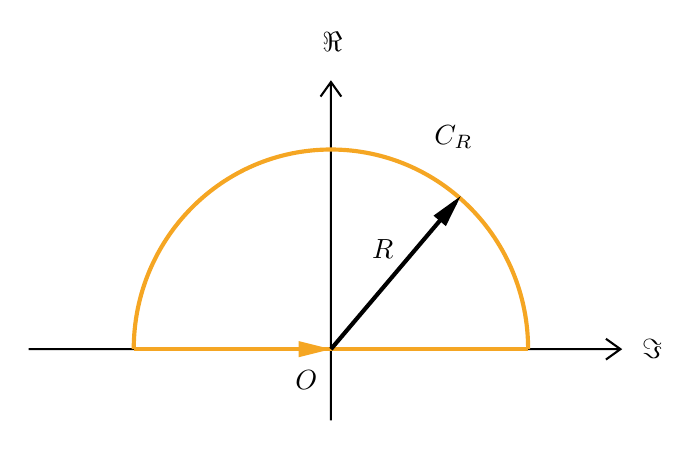
\begin{tikzpicture}[x=0.75pt,y=0.75pt,yscale=-1,xscale=1]
%uncomment if require: \path (0,266); %set diagram left start at 0, and has height of 266

%Shape: Axis 2D [id:dp1282392211894816] 
\draw  (162,181.79) -- (447.09,181.79)(307.61,53.09) -- (307.61,216.09) (440.09,176.79) -- (447.09,181.79) -- (440.09,186.79) (302.61,60.09) -- (307.61,53.09) -- (312.61,60.09)  ;
%Shape: Arc [id:dp1814309272431356] 
\draw  [draw opacity=0][line width=1.5]  (212.6,181.79) .. controls (212.6,181.79) and (212.6,181.79) .. (212.6,181.79) .. controls (212.6,128.66) and (255.14,85.6) .. (307.61,85.6) .. controls (360.08,85.6) and (402.61,128.66) .. (402.61,181.79) -- (307.61,181.79) -- cycle ; \draw  [color={rgb, 255:red, 245; green, 166; blue, 35 }  ,draw opacity=1 ][line width=1.5]  (212.6,181.79) .. controls (212.6,181.79) and (212.6,181.79) .. (212.6,181.79) .. controls (212.6,128.66) and (255.14,85.6) .. (307.61,85.6) .. controls (360.08,85.6) and (402.61,128.66) .. (402.61,181.79) ;  
%Straight Lines [id:da15038694853465828] 
\draw [color={rgb, 255:red, 245; green, 166; blue, 35 }  ,draw opacity=1 ][line width=1.5]    (212.6,181.79) -- (402.61,181.79) ;
\draw [shift={(307.61,181.79)}, rotate = 180] [fill={rgb, 255:red, 245; green, 166; blue, 35 }  ,fill opacity=1 ][line width=0.08]  [draw opacity=0] (15.6,-3.9) -- (0,0) -- (15.6,3.9) -- cycle    ;
%Straight Lines [id:da12449754393780421] 
\draw [color={rgb, 255:red, 0; green, 0; blue, 0 }  ,draw opacity=1 ][line width=1.5]    (307.61,181.79) -- (352.62,128.69) -- (367.5,111.14) ;
\draw [shift={(370.09,108.09)}, rotate = 130.29] [fill={rgb, 255:red, 0; green, 0; blue, 0 }  ,fill opacity=1 ][line width=0.08]  [draw opacity=0] (15.6,-3.9) -- (0,0) -- (15.6,3.9) -- cycle    ;


% Text Node
\draw (289,190.4) node [anchor=north west][inner sep=0.75pt]    {$O$};
% Text Node
\draw (302,27.4) node [anchor=north west][inner sep=0.75pt]    {$\Re $};
% Text Node
\draw (456,175.4) node [anchor=north west][inner sep=0.75pt]    {$\Im $};
% Text Node
\draw (326,127.4) node [anchor=north west][inner sep=0.75pt]    {$R$};
% Text Node
\draw (356,72.4) node [anchor=north west][inner sep=0.75pt]    {$C_{R}$};

% \draw   (239.6, 212.79) circle [x radius= 5, y radius= 5]  (234.6,212.79) -- (244.6,212.79)(239.6,207.79) -- (239.6,217.79) ;
% \draw   (334.61, 116.6) circle [x radius= 5, y radius= 5]  (329.61,116.6) -- (339.61,116.6)(334.61,111.6) -- (334.61,121.6) ;
% \draw   (429.61, 212.79) circle [x radius= 5, y radius= 5]  (424.61,212.79) -- (434.61,212.79)(429.61,207.79) -- (429.61,217.79) ;
% \draw   (396.48, 139.8) circle [x radius= 5, y radius= 5]  (391.48,139.8) -- (401.48,139.8)(396.48,134.8) -- (396.48,144.8) ;
\end{tikzpicture}


\begin{figure}[htb!]
    \centering
    


\tikzset{every picture/.style={line width=0.75pt}} %set default line width to 0.75pt        

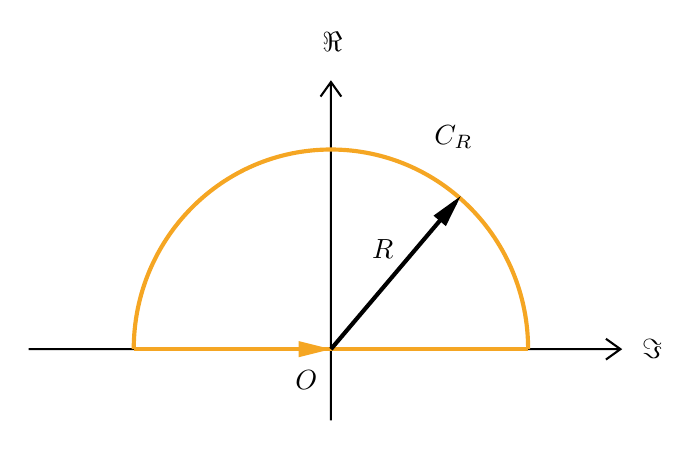
\begin{tikzpicture}[x=0.75pt,y=0.75pt,yscale=-1,xscale=1]
%uncomment if require: \path (0,266); %set diagram left start at 0, and has height of 266

%Shape: Axis 2D [id:dp1282392211894816] 
\draw  (162,181.79) -- (447.09,181.79)(307.61,53.09) -- (307.61,216.09) (440.09,176.79) -- (447.09,181.79) -- (440.09,186.79) (302.61,60.09) -- (307.61,53.09) -- (312.61,60.09)  ;
%Shape: Arc [id:dp1814309272431356] 
\draw  [draw opacity=0][line width=1.5]  (212.6,181.79) .. controls (212.6,181.79) and (212.6,181.79) .. (212.6,181.79) .. controls (212.6,128.66) and (255.14,85.6) .. (307.61,85.6) .. controls (360.08,85.6) and (402.61,128.66) .. (402.61,181.79) -- (307.61,181.79) -- cycle ; \draw  [color={rgb, 255:red, 245; green, 166; blue, 35 }  ,draw opacity=1 ][line width=1.5]  (212.6,181.79) .. controls (212.6,181.79) and (212.6,181.79) .. (212.6,181.79) .. controls (212.6,128.66) and (255.14,85.6) .. (307.61,85.6) .. controls (360.08,85.6) and (402.61,128.66) .. (402.61,181.79) ;  
%Straight Lines [id:da15038694853465828] 
\draw [color={rgb, 255:red, 245; green, 166; blue, 35 }  ,draw opacity=1 ][line width=1.5]    (212.6,181.79) -- (402.61,181.79) ;
\draw [shift={(307.61,181.79)}, rotate = 180] [fill={rgb, 255:red, 245; green, 166; blue, 35 }  ,fill opacity=1 ][line width=0.08]  [draw opacity=0] (15.6,-3.9) -- (0,0) -- (15.6,3.9) -- cycle    ;
%Straight Lines [id:da12449754393780421] 
\draw [color={rgb, 255:red, 0; green, 0; blue, 0 }  ,draw opacity=1 ][line width=1.5]    (307.61,181.79) -- (352.62,128.69) -- (367.5,111.14) ;
\draw [shift={(370.09,108.09)}, rotate = 130.29] [fill={rgb, 255:red, 0; green, 0; blue, 0 }  ,fill opacity=1 ][line width=0.08]  [draw opacity=0] (15.6,-3.9) -- (0,0) -- (15.6,3.9) -- cycle    ;


% Text Node
\draw (289,190.4) node [anchor=north west][inner sep=0.75pt]    {$O$};
% Text Node
\draw (302,27.4) node [anchor=north west][inner sep=0.75pt]    {$\Re $};
% Text Node
\draw (456,175.4) node [anchor=north west][inner sep=0.75pt]    {$\Im $};
% Text Node
\draw (326,127.4) node [anchor=north west][inner sep=0.75pt]    {$R$};
% Text Node
\draw (356,72.4) node [anchor=north west][inner sep=0.75pt]    {$C_{R}$};

% \draw   (239.6, 212.79) circle [x radius= 5, y radius= 5]  (234.6,212.79) -- (244.6,212.79)(239.6,207.79) -- (239.6,217.79) ;
% \draw   (334.61, 116.6) circle [x radius= 5, y radius= 5]  (329.61,116.6) -- (339.61,116.6)(334.61,111.6) -- (334.61,121.6) ;
% \draw   (429.61, 212.79) circle [x radius= 5, y radius= 5]  (424.61,212.79) -- (434.61,212.79)(429.61,207.79) -- (429.61,217.79) ;
% \draw   (396.48, 139.8) circle [x radius= 5, y radius= 5]  (391.48,139.8) -- (401.48,139.8)(396.48,134.8) -- (396.48,144.8) ;
\end{tikzpicture}


    \caption{半圆路径.}
    \label{fig:semicircle}
\end{figure}
下面证明上式第二项为零.一般的对于任意$\theta_1 \leq \theta \leq \theta_2$, 
有$\lim_{R\to \infty} zf(z) = 0$,可以证明对于该角度对应的圆弧$C$有,
\begin{equation}
    \lim_{R \rightarrow \infty} \int_C f(z) dz = 0 .
\end{equation}

\[
    \begin{aligned}
    \lim _{R \rightarrow \infty}\left|\int_C f(z) d z\right| \leq \int_{\theta_1}^{\theta_2} \lim _{R \rightarrow \infty}\left|f\left(R e^{i \theta}\right) i R e^{i \theta}\right| & d \theta \\
    & \leq\left(\theta_2-\theta_1\right) \lim _{R \rightarrow \infty}\left|f\left(R e^{i \theta}\right) R e^{i \theta}\right|=0 .
    \end{aligned}
\]
也就是说,
\begin{equation}
    \int_{-R}^R f(x) d x = 2\pi \imath  \sum_{z_j\in \textrm{上半平面}} \Res f(z_j),
\end{equation}

\begin{examplebox}{计算\[ 
    I = \int_{-\infty}^{\infty} \frac{dx}{1 + x^2}   .
    \]}
    由$f(z) = \frac{1}{1+ x^2} = \frac{1}{(z-\imath)(z+\imath)}$可知
    其单极点$\pm \imath$,其中$\imath$在上半平面.
    \[
      \Res f(+\imath) = \frac{1}{2\imath}  
    \]
    因此,$I = 2\pi \imath  \frac{1}{2\imath} = \pi$.由于该积分是一个常见积分
    亦可以通过原函数$\arctan(x)$得到.留数定理的还可以计算这样的积分,
    \[
      I\int_{-\infty}^{\infty} \frac{dx}{(1 + x^2)^n} 
    \]
    具体求解过程参考梁昆淼数学物理方法的解.
\end{examplebox}


 \subsection{带复指数的定积分}
 考虑以下类型的定积分
 \begin{equation}
    I=\int_{-\infty}^{\infty} f(x) e^{\imath m x} d x
\end{equation}
其中,$m$为正实数;$f(z)$在上半平面除有限个奇点外是解析的,且$\lim_{|z|\to \infty} f(z) = 0, 0 \leq arg z \leq \pi$.
我们使用同样的半圆路径,类似的可以通过留数定理将实轴的积分转换为环路积分求得.
为了使用留数定理,我们先需要证明在半圆上的路径积分为零,这里就要用到\textbf{约旦引理}(Jordan lemma
).
即证明
\begin{equation}
    \lim _{R \rightarrow \infty} \int_{C_R} f(z) e^{\imath m z} d z=0 .
\end{equation}
当$R$足够大时,我们有$|f(z)| < \epsilon$.半圆积分
\begin{align}
    I_R&=\int_0^\pi f\left(R e^{\imath \theta}\right) 
    e^{\imath m R \cos \theta- m R \sin \theta} \imath R e^{\imath \theta} d \theta
    \\
    &\leq \epsilon R \int_0^\pi e^{-m R \sin \theta} d \theta=2 \epsilon R \int_0^{\pi / 2} e^{-m R \sin \theta} d \theta,
\end{align}
可以发现在$\left[ 0, \pi/2\right]$时,
\begin{equation}
    \frac{2}{\pi}\theta \leq \sin{\theta},
\end{equation}
于是有
\begin{equation}
    I_R \leq 2 \epsilon R \int_0^{\pi / 2} e^{-2 m R \theta / \pi} d \theta=2 \epsilon R \frac{1-e^{-m R}}{2 m R / \pi}<\frac{\pi}{m} \epsilon
\end{equation}
即
\begin{equation}
    \lim_{R\to \infty} I_R = 0.
\end{equation}
回到定积分$I$,可以得
\begin{equation}
    \label{eq:complex_exponential_integral}
    I=\int_{-\infty}^{\infty} f(x) e^{ \imath m x} d x = 2\pi \imath \sum_{z_j \in \text{上半平面}} \Res e^{\imath m z_j} f(z_j)
\end{equation}

对于以下类型的积分,可以利用上述结论.如
\begin{equation}
    \int_{0}^{\infty} f(x) \cos {m x} dx, \int_{0}^{\infty} G(x) \sin{m x} dx
\end{equation}
其中,$F(z)$为偶函数,$G(z)$为奇函数,它们在实轴上没有奇点,上半平面上除有限个奇点外解析.
很容易通过$\cos{mx} = \frac{1}{2}\left( e^{\imath m x} + e^{-\imath mx}\right)$等变换得到,即
$$
\begin{aligned}
\int_0^{\infty} F(x) \cos m x d x & =\int_0^{\infty} F(x) \frac{1}{2}\left(e^{\imath m x}+e^{-\imath m x}\right) \mathrm{d} x \\
& =\frac{1}{2} \int_0^{\infty} F(x) e^{\imath m x} d x+\frac{1}{2} \int_0^{\infty} F(x) e^{-\imath m x} d x 
\\
& = \frac{1}{2} \int_{-\infty}^{\infty} F(x) e^{\imath m x} d x. 
\end{aligned}
$$

\begin{examplebox}{计算 $\int_0^{\infty} \frac{\cos m x}{x^2+a^2} d x$.}
偶函数$F(z) e^{\imath m z}=\frac{1}{z^2+a^2} e^{\imath m z}$ 有两个单极点 $\pm a \imath$, 其中 $+a \imath$ 在上半平面. 而 $e^{\imath m z} /\left(z^2+a^2\right)$ 在单极点 $+a \imath$ 的留数为
    $$
    \lim _{z \rightarrow a \imath}\left[(z-a \imath) \frac{e^{\imath m z}}{z^2+a^2}\right]=\lim _{z \rightarrow a \imath}\left[\frac{e^{\imath m z}}{z+a \imath}\right]=\frac{e^{-m a}}{2 a \imath}
    $$
    应用\ref{eq:complex_exponential_integral},
    $$
    \int_0^{\infty} \frac{\cos m x}{x^2+a^2} d x=\pi \imath \frac{e^{-m a}}{2 a \imath}=\frac{\pi}{2 a} e^{-m a}.
    $$
\end{examplebox}